\documentclass{article}
\usepackage[utf8]{inputenc}
\usepackage{amsmath}
\usepackage{amsfonts}
\usepackage{graphicx}
\usepackage{amssymb}
\usepackage{amsthm}
\usepackage{float}
\usepackage{tikz}
\usepackage{mlmodern}
\usepackage{subfig}
\usepackage[T1]{fontenc}
\usepackage[left=2.5cm,right=2.5cm]{geometry}
\usepackage[linesnumbered,ruled]{algorithm2e}

\usepackage{svg}

\usepackage{listings}
\newcommand{\code}[1]{\texttt{#1}} % inline code setting
\renewcommand{\lstlistingname}{Code}

\definecolor{codebg}{RGB}{230,230,230}
\lstset {
    breakatwhitespace=false,         % sets if automatic breaks should only happen at whitespace
    breaklines=true,                 % sets automatic line breaking
    captionpos=b,                    % sets the caption-position to bottom
    tabsize=4,
    %showstringspaces=false,
    numbers=left,                    % where to put the line-numbers; possible values are (none, left, right)
    numbersep=2pt,                   % how far the line-numbers are from the code
    numberstyle=\tiny, % the style that is used for the line-numbers
    %upquote=true,
    backgroundcolor = \color{codebg},
    basicstyle=\small\ttfamily, % basic font setting
    emph={int,char,double,float,unsigned,void,bool},
    %emphstyle={\color{blue}},
    escapechar=\&,
    columns=fixed
}

\newtheorem{defi}{Definition}
\newtheorem{ex}{Example}
\newtheorem{prop}{Proposition}
\newtheorem{theorem}{Theorem}
\newtheorem{lemma}{Lemma}
\newtheorem{kor}{Corollary}

\newcommand{\N}{\mathbb{N}}

\newcommand{\R}{\mathbb{R}}
\newcommand{\V}{\mathcal{V}}
\newcommand{\E}{\mathcal{E}}

\title{\texttt{maniflow} -- a (partial) documentation}
\author{Felix Widmaier}
\date{}


\begin{document}
\maketitle
\section{Introduction}
\begin{defi}[Mesh]
    Let $V$ be a vector space  over $\R$ of dimension $n$. Let $\mathcal{V}_M\subset V$ be a set of points in $V$. We further let $\mathcal{F}_M\subset\mathcal{V}_M^3$. The pair $M = (\mathcal{V}_M, \mathcal{F}_M)$ is then called mesh. The elements of $\mathcal{V}_M$ are called points of $M$ and the elements of $\mathcal{F}_M$ are the faces of the mesh $M$.
\end{defi}
For a mesh $M = (\mathcal{V}_M, \mathcal{F}_M)$ we will often denote $V_M = \vert\mathcal{V}_M\vert$ and $F_M = \vert\mathcal{F}_M\vert$.
\paragraph{Remark.} Meshes $M$ can be considered as $2$-dimensional simplicial complexes. Thus for $2$-dimensional manifolds $\Tilde{M}\subset V$ we may find a \textit{triangulation} simplicial complex $K$ of $\Tilde{M}$. The corresponding mesh will be called \textit{triangulation} mesh of the manifold $\Tilde{M}$.
\begin{ex}[Tetrahedron] Let 
\begin{align*}
    \mathcal{V} = \left\{\left(\sqrt{\frac89},0,-\frac13\right),\left(-\sqrt{\frac29},\sqrt{\frac23},-\frac13\right),\left(-\sqrt{\frac29},-\sqrt{\frac23},-\frac13\right), \left(0,0,1\right)\right\}\subset\R^3
\end{align*}
and $\mathcal{F} = \{f\in2^{\mathcal{V}}:\vert f\vert = 3\}$. The mesh $T = (\mathcal{V},\mathcal{F})$ is the tetrahedron, which is displayed in figure \ref{fig:tetra}.
    \begin{figure}[h]
        \centering
        \includesvg[scale=0.6]{img/tetrahedron.svg}
        \caption{Tetrahedron}
        \label{fig:tetra}
    \end{figure}
This can be implemented using \texttt{maniflow} by using the \texttt{Mesh} class:
\begin{lstlisting}
import numpy as np
import itertools
from maniflow.mesh import Mesh, Face

# computing the four vertices of the tetrahedron
v1 = np.array([np.sqrt(8/9), 0, -1/3])
v2 = np.array([-np.sqrt(2/9), np.sqrt(2/3), -1/3])
v3 = np.array([-np.sqrt(2/9), -np.sqrt(2/3), -1/3])
v4 = np.array([0, 0, 1])

tetra = Mesh()
# setting the vertices as the vertices of the new mesh object
tetra.vertices = [v1, v2, v3, v4]
# now we compute the subsets of all the vertices consiting of three vertices
subsets = set(itertools.combinations(list(range(tetra.v)), 3))
# the faces are then set as the faces of tetra
tetra.faces = [Face(tetra, *list(i)) for i in subsets]
\end{lstlisting}
This way, we obtain the \texttt{Mesh} object \texttt{tetra} which represents a tetrahedron.
\end{ex}
\begin{defi}[Undirected Graph]
    Let $\V_G$ be a set and $\E_G\subset\{e\in2^{\V_G}: |e|=2\}$ be a set of unordered pairs of elements from $\V_G$. The pair $G = (\V_G, \E_G)$ is then called undirected Graph. The elements from $\V_G$ are called vertices of $G$ and the elements from $\E_G$ are called edges of $G$.
\end{defi}
For a Graph $G=(\V_G,\E_G)$ we write
\begin{align*}
    \vcenter{\hbox{\begin{tikzpicture}
    \node (A) at (0,0) {$x$};
    \node (B) at (1,0) {$y$};
    \draw[-] (A) -- (B);\end{tikzpicture}}}
\end{align*}
if $\{x,y\}\in\E_G$. If we take all edges and points together in this way, we get the picture
of a graph with undirected edges.
\begin{ex}
    \begin{equation}\label{eq:sample_g}
    G\colon\left(\vcenter{\hbox{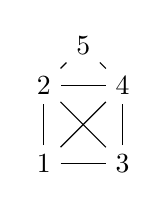
\begin{tikzpicture}[scale=0.5]
    \node (1) at (-1,-1) {$1$};
    \node (2) at (-1,1) {$2$};
    \node (3) at (1,-1) {$3$};
    \node (4) at (1,1) {$4$};
    \node (5) at (0,2) {$5$};
    \draw[-] (1) -- (2);
    \draw[-] (2) -- (3);
    \draw[-] (3) -- (4);
    \draw[-] (4) -- (2);
    \draw[-] (2) -- (5);
    \draw[-] (5) -- (4);
    \draw[-] (4) -- (1);
    \draw[-] (1) -- (3);
\end{tikzpicture}}}\right),\qquad H\colon\left(\vcenter{\hbox{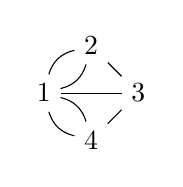
\begin{tikzpicture}[scale=0.6]
\node (1) at (-1, 0) {$1$};
\node (2) at (0, 1) {$2$};
\node (3) at (1,0) {$3$};
\node (4) at (0,-1) {$4$};
\draw[-] (1) -- (3);
\path [-] (1) edge[bend right=-30](2); 
\path [-] (1) edge[bend right=30](2); 
\path [-] (1) edge[bend right=-30](4); 
\path [-] (1) edge[bend right=30](4);
\draw[-] (3) -- (2);
\draw[-] (4) -- (3);
\end{tikzpicture}}}\right)
\end{equation}
\end{ex}
\begin{defi}[Face Graph]
    Let $M = (\mathcal{V}_M, \mathcal{F}_M)$ be a mesh and
    \begin{align*}
        \mathcal{E} = \left\{(f_1,f_2)\in\mathcal{F}_G^2: \vert f_1\cap f_2\vert =2\right\}
    \end{align*}
    The face graph of $M$ is the graph $(\mathcal{F}_M,\mathcal{E})$.
\end{defi}
\begin{ex} The face graph of the tetrahedron is given by
    \begin{equation}\label{eq:sample_g}
    G\colon\left(\vcenter{\hbox{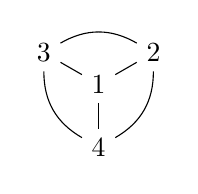
\begin{tikzpicture}[scale=0.8]
    \node (1) at (0,0) {$1$};
    \node (2) at (0.87,0.5) {$2$};
    \node (3) at (-0.87,0.5) {$3$};
    \node (4) at (0,-1) {$4$};
    \draw[-] (1) -- (2);
    \draw[-] (1) -- (3);
    \draw[-] (1) -- (4);
    \path[-] (2) edge[bend right=30] (3);
    \path[-] (3) edge[bend right=30] (4);
    \path[-] (4) edge[bend right=30] (2);
\end{tikzpicture}}}\right)
\end{equation}
\end{ex}
The face graph of a given mesh can be constructed by algorithm \ref{alg:facegraph}.
\begin{algorithm}\label{alg:facegraph}
    \SetKwInOut{Input}{Input}
    \SetKwInOut{Output}{Output}

    \Input{A mesh $M = (\mathcal{V}_M, \mathcal{F}_M=\{f_1,f_2,f_3\ldots\})$}
    \Output{The adjacency matrix of the face graph of the mesh $M$}
    \caption{Construction of the face graph of a given mesh}
    $G := 0\in\R^{F_M\times F_M}$\;
    \For{$i=1$ \KwTo $F_M$}
    {
        $neighbors := 0$\;
        \For{$j=1$ \KwTo $F_M$}
        {
            \If{$neighbors = 3$}{
            \textbf{break}\;
            }
            \If{$\vert f_i\cap f_j\vert = 2$ \normalfont{\textbf{and}} $i\neq j$}{
            $G_{ij} \leftarrow 1$\;
            $neighbors \leftarrow neighbors + 1$\;
            }
        }
    }
    \Return{$G$}
\end{algorithm}
Since this algorithm loops over the faces of the mesh in a nested way, the complexity of it lies in $O(F_M^2)$. As this runtime complexity has the consequence of the algorithm being very slow at execution for somewhat large meshes, the face graph is computed dynamically by \texttt{maniflow.mesh.Mesh.faceGraph}.
\newpage
\subsection{A first application: \texttt{maniflow.mesh.utils.connectedComponents}}
The method \texttt{maniflow.mesh.utils.connectedComponents} decomposes the given mesh into its connected components. Now that we have an algorithm with which to compute the face graph, the connected components of a mesh can now be identified as the connected components of the face graph. These can be determined via the breadth-first traversal of the face graph. 
\begin{algorithm}\label{alg:components}
    \SetKwInOut{Input}{Input}
    \SetKwInOut{Output}{Output}

    \Input{A mesh $M = (\mathcal{V}_M, \mathcal{F}_M=\{f_1,f_2,f_3\ldots\})$}
    \Output{The connected components of the mesh $M$}
    \caption{Construction of the face graph of a given mesh}
    Compute the adjacency matrix $G$ using \ref{alg:facegraph}\;
    $start := 1$\;
    $n := 1$\;
    \While{$\mathcal{F}_M\neq\emptyset$}{
        Compute a breadth first traversal sequence $T_n \leftarrow \{f_{start}, f_b,f_c,\ldots\}\subseteq\mathcal{F}_M$\;
        $n \leftarrow n+1$\;
        $\mathcal{F}_M\leftarrow \mathcal{F}_M\setminus T_n$\;
        Set $1< start\leq F_M$ such that $f_{start}\in\mathcal{F}_M$\;
    }
    
    \Return{$T_1$, $T_2$, $\ldots$}
\end{algorithm}
\paragraph{Runtime analysis.} The algorithm \ref{alg:facegraph} has a runtime complexity which lies in $O(F_M^2)$. The breadth-first traversal on the face graph has a runtime\footnote{Since on a graph with the number of vertices being $V$ and the number of edges being $E$ the breadth first search has a complexity of $O(E + V)$. As every face has at most three neighbors we obtain the given runtime complexity.} complexity of $O(F_G + 3\cdot F_G) = O(F_G)$. The computation of $\mathcal{F}_M\setminus T_n$ has also quadratic complexity $O(\vert\mathcal{F}_M\vert^2)$. Thus the overall complexity of algorithm \ref{alg:components} lies in $O(F_G^2)$.
\begin{ex}
    In this example we analyse the connected components of the teapot from \texttt{examples/teapot.obj}. The teapot is displayed in figure \ref{fig:teapot}.
    \begin{figure}[h]
        \centering
        \includegraphics[scale=0.15]{img/teapot.png}
        \caption{The teapot from \texttt{examples/teapot.obj}}
        \label{fig:teapot}
    \end{figure}
    \newline\noindent The connected components can be computed using the following code
    \begin{lstlisting}
from maniflow.mesh import Mesh
from maniflow.mesh.obj import OBJFile
from maniflow.mesh.utils import connectedComponents, coincidingVertices

teapot = OBJFile.read("examples/teapot.obj")
coincidingVertices(teapot)
components = connectedComponents(teapot)

for i, component_list in enumerate(components):
    component = Mesh.fromFaceList(teapot, *component_list)
    OBJFile.write(component, "teapot" + str(i + 1) + ".obj")
    \end{lstlisting}
    \begin{figure}[ht]
    \centering
    \subfloat[The lid of the teapot]{\includegraphics[width=0.4\textwidth]{img/teapot1.png}}\hfil
    \subfloat[The handle of the teapot]{\includegraphics[width=0.4\textwidth]{img/teapot2.png}}\hfil\\
    \subfloat[The body of the teapot]{\includegraphics[width=0.4\textwidth]{img/teapot3.png}}\hfil
    \subfloat[The spout of the teapot]{\includegraphics[width=0.4\textwidth]{img/teapot4.png}}\hfil
    \caption{The connected components of the teapot}
    \label{fig:einsteinex}
\end{figure}
\end{ex}
\end{document}
